\section*{\textbf{Empirical Application}}

\subsection*{ICEWS Material Conflict}

A number of projects have arisen seeking to create large data sets of dyadic events through the automatic extraction of information from on-line news archives. This has made it empirically easier to study interactions among countries, as well as among actors such as NGOs within countries.

The two most well-known developments include the ICEWS event data project \citep{icews:2015:data} and the Phoenix pipeline \citep{oeda:2016}. For the purposes of this project we focus on utilizing the ICEWS database as it extends back farther in time. ICEWS draws from over 300 different international and national focused publishers \citep{boschee:etal:2015}. The ICEWS event data are based on a continuous monitoring of over 250 news sources and other open source material covering 177 countries worldwide. ICEWS consists of several components, including a database of over 38 million multilingual news stories going back to 1990 and present to last week. The ICEWS data along with extensive documentation have been made publicly available (with a one year embargo) on \url{dataverse.org} \citep{icews:2015:aggregations,icews:2015:data}. To classify news stories into socio-political topics, ICEWS relies on a augmented and expanded version of the CAMEO coding scheme \citep{schrodt:etal:2009}. The dictionaries, aggregations, ground truth data, and actor and verb dictionaries are publicly  available with a one year lag at the ICEWS data repository \url{https://dataverse.harvard.edu/dataverse/icews}. In addition,  the event coder has been made available publicly by the Office of the Director of National Intelligence.\footnote{Details at \url{http://bit.ly/2nS4nBU}.} This event coder, known as ACCENT, searches for the following information: a sender, a receiver, an action type, and a time stamp. The set of action types covered include activities between dyads such as ``Occupy territory'', ``Use conventional force'', and ``Impose embargo, boycott, or sanctions''. Then, the ontology provides rules through which the parsed story is coded. An example of a coded news story fitting this last category is:

\begin{quote}
	``\textit{President Bill Clinton has imposed sanctions on the Taliban religious faction that controls Afghanistan for its support of suspected terrorist Osama bin Laden, the White House said Tuesday.}''
\end{quote}

In this example, the actor designated as sending the action is the United States and the actor receiving it is Afghanistan. Dyadic measurements such as these are available for 249 countries, and the dataset is updated regularly. Currently, data up until March 2016 has been made publicly available on the ICEWS dataverse.

Our sample for this analysis focuses on monthly level interactions between countries in the international system from 2005 to 2012.\footnote{The ICEWS data extends to 2016 but we end at 2012 due to temporal coverage constraints among other covariates that we have incorporated into the model.} To measure conflict from this database we focus on what is often referred to as the ``material conflict'' variable. This variable is taken from the ``quad variable'' framework developed by \citet{duval:thompson:1980}. \citet{schrodt:yonamine:2013} defines the type of events that get drawn into this category as those involving, ``Physical acts of a conflictual nature, including armed attacks, destruction of property, assassination, etc.''.

\newcolumntype{M}[1]{>{\centering\arraybackslash}m{#1}}
\begin{figure}[ht]
	\centering
	\hspace{-80mm}
	\begin{tabular}{M{1cm}M{2.5cm}}
	    \scshape{January 2005} & 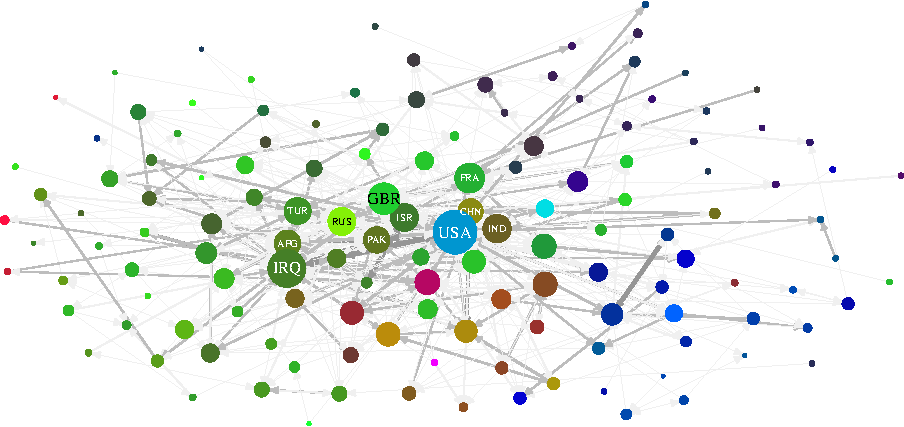
\includegraphics[width=.8\textwidth]{figure4_jan05.pdf}  \\
	    \scshape{December 2012} & 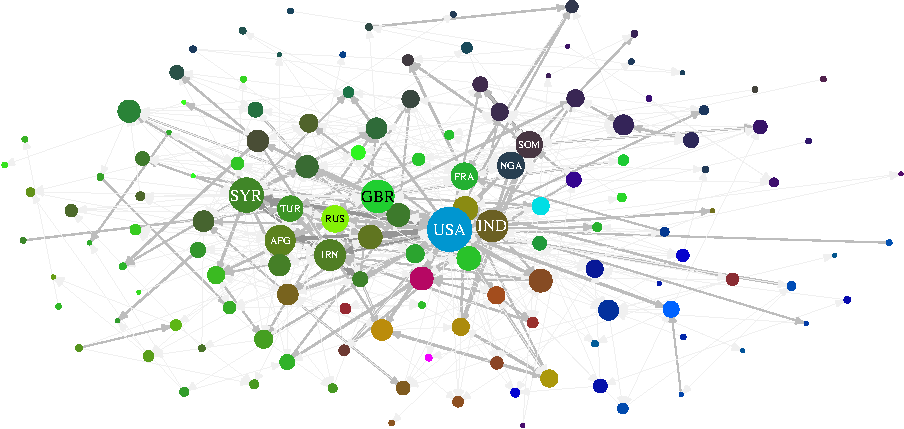
\includegraphics[width=.8\textwidth]{figure4_dec12.pdf} \\
	    \multicolumn{2}{c}{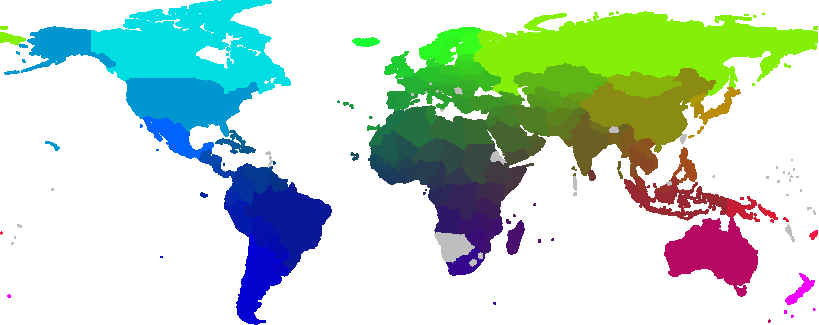
\includegraphics[width=.4\textwidth]{map.pdf}} \\
	\end{tabular}
	\caption{Network depiction of ICEWS Material Conflict events for January 2005 (top) and December 2012 (bottom).}
	\label{fig:icews}
\end{figure}
\FloatBarrier

Figure~\ref{fig:icews} visualizes the material conflict variable as a network, specifically, we provide snapshots of events between dyads along this relational dimension in January 2005 and December 2012. The size of the nodes correspond to how active countries are in the network, and each node is colored by its geographic position. An edge between two nodes designates that at least one material conflict event has taken place between that dyad, and arrows indicate the sender and receiver. Thicker edges indicate a greater count of material conflict events between a dyad.

In both snapshots, the United States is highly involved in conflict events occurring in the system both in 2005 and 2012. Additionally, other major powers such as Russia and the Great Britain are also frequently involved. Some notable changes are visible in the network. While in 2005 Iraq was highly involved in material conflict events by 2012 Syria became more active. Last, there is a significant amount of clustering by geography in this network. Conflict involving Latin American countries is relatively infrequent but when it does occur, it seems to primarily involve countries within the region.

\subsection*{Parameters with direct effect}

We first parameterize the model by identifying variables that we hypothesize have a direct impact on material conflict patterns between countries. There are a number of the standard explanations provided in the conflict literature. Inertia and reprocity top the list. Conflict in period $t$ is affected by what occurred previously in period $t-1$. This is autoregressive dependence. The expectation is that a dyad engaged in conflict in the previous period is more likely to be engaged in conflict in the next.

A lagged reciprocity parameter embodies the common argument that if country $j$ receives conflict from $i$ in period $t$, that in period $t+1$ $j$ may retaliate by sending conflict to $i$. The argument that reciprocity is likely to occur in conflict networks is certainly not novel, and has its roots in well known theories involving cooperation and conflict between states \citep{richardson:1960,choucri:north:1972,goldstein:1992}.

A number of exogenous explanations have often been used to explain conflicts between dyads. One of the most common relates to the role of geography. Apart from conflict involving major powers, conflict between countries that are geographically proximate is typical \citep{bremer:1992,diehl:goertz:2000,carter:goemans:2011}. Figure~\ref{fig:icews} demonstrates evidence of regional conflict patterns, as indicated by the clustering of similarly colored nodes, which represent countries within the same geographic region. This clustering suggests that conflicts are more likely to occur between countries in the same region. We use the minimum, logged distance between the dyads to operationalize this explanation.\footnote{Minimum distance estimation was conducted using the \pkg{CShapes} package \citep{weidmann:etal:2010a}.}

One of the most well developed arguments linking conflict between dyads to domestic institutions involves the idea of the democratic peace. The specific vein of this argument that has found the most support is the idea that democracies are unlikely to go to war with one another \citep{small:singer:1976,maoz:abdolali:1989,russett:oneal:2001}. Arguments for why democracies may have more peaceful relations between themselves range from how they share certain norms that make them less likely to engage in conflict to others hypothesizing that democratic leaders are better able to demonstrate resolve thus reducing conflict resulting from incomplete information \citep{maoz:russett:1993,fearon:1995}. To operationalize this argument, we construct a binary indicator that is one when both countries in the dyad are democratic.\footnote{We define a country as democratic if its polity score is greater than or equal to seven according to the Polity IV project \citep{marshall:jaggers:2002}.}

We also control for whether or not a pair of countries are allied to one another using data from the Correlates of War \citep{gibler:sarkees:2004}.\footnote{We consider a pair of countries allied to one another if they share a mutual defense treaty, neutrality pact, or entente.} Typically, one would expect that states allied to one another are less likely to engage in conflict. Another common control in the conflict literature is the level of trade between a pair of countries. We estimate trade flows between countries using the International Monetary Fund (IMF) Direction of Trade Statistics \citep{imf:2012}. Incorporating the level of trade between countries speaks to a long debate on the role that economic interdependencies may play in mitigating the risk of conflict between states \citep{barbieri:1996,gartzke:etal:2001}.\footnote{The extant literature has employed a variety of parameterizations to test this hypothesis. At times, a measure of trade dependence is calculated and at others just a simple measure of the trade flows between a pair of countries. We show results for the latter parameterization but results are consistent if we utilize a measure of trade dependence.}

The last set of measures we use to predict dyadic conflict are derived from another ICEWS quad variable. Verbal cooperation counts the occurrence of statements expressing a desire to cooperate from one country to another.\footnote{An example of a verbal cooperation event sent from Turkey to Portugal is the following: ``\textit{Portugal will support Turkey's efforts to become a full member of the European Community, Portuguese President Mario Soares said on Tuesday}.''}  We include a lagged and reciprocal version of this variable to our specification. This monthly level measure of cooperation between states provides us with a thermometer measure of the relations between states that is measured at a low level of temporal aggregation.

\subsection*{Parameters defining influence patterns}

We next add covariates to the model to explain the influence patterns observed in the network. The SIR model introduces the ability to explain these patterns using an underlying regression model, which is jointly estimated with the parameters modeling $y_{ij}$ through the iterative procedure described earlier. Using the SIR model we can answer the following types of questions:

\begin{itemize}
    \item Do the actions of one country at time $t-1$ influence the actions directed towards another country at time $t$ within the network, as reflected in the influence parameters $a_{ii'}$ and $b_{jj'}$?
	\item Which factors explain the network effects embedded in the influence parameters $a_{ii'}$ and $b_{jj'}$, determining the impact of one country's actions at time $t-1$ on the subsequent actions towards another country at time $t$?
\end{itemize}

The first covariate added to the influence specification, is simply a control for the distance between countries.\footnote{This is operationalized similarly as above using data from \pkg{CShapes}.} A negative effect for the distance parameter in the case of sender influence would indicate that countries are likely to send conflictual actions to the same countries that their neighbors are sending conflictual actions too. In the case of receiver influence, a negative effect would indicate that countries are likely to be targeted by the same set of countries that their neighbors are receiving conflictual interactions from.

An argument that has received continuing attention in the political science literature is the role that alliances play in either mitigating or exacerbating the level of conflict in the international system. Some have argued that in the case of a conflict, a country's allies will join in to honor their commitments thus increasing the risks for a multiparty interstate conflict \citep{snyder:1984,leeds:2003,vasquez:rundlett:2016}. We would find evidence for this argument if the ally parameter in the case of sender influence was positive, as that would indicate that countries are more likely to initiate or increase the level of conflict with countries that their allies are in conflict with.

The next covariate we consider is the volume of trade between countries. Trade relationships are often seen as a stabilizing factor in international relations, under the premise that economic interdependence reduces the likelihood of conflict by raising the costs of disruption \citep{keohane:nye:1977,oneal:russett:1999}. In the context of sender influence, a negative effect for the trade parameter would suggest that countries are less likely to initiate conflict with the same targets as their trading partners, supporting the idea that trade can act as a deterrent to conflict. Conversely, in the case of receiver influence, a positive effect would indicate that countries receiving conflict from others may also be the targets of those same countries' trading partners, potentially due to tensions arising from competitive trade dynamics.

The final covariate we examine is the level of verbal cooperation between countries, as indicated by diplomatic communications or public statements of support. Verbal cooperation can signal strong diplomatic ties or shared interests, potentially influencing patterns of conflict and cooperation in the network \citep{dorussen:ward:2008}. In the case of sender influence, a positive effect for the verbal cooperation parameter would imply that countries are more likely to align their conflictual actions with those of countries with whom they have a high degree of verbal cooperation, possibly as a show of solidarity or shared strategy. For receiver influence, a positive effect would suggest that countries facing conflict from one state may also find themselves targeted by that state's verbal allies, indicating a broader alignment in the international system.

Table~\ref{tab:modspec} summarizes each of the covariates used to estimate the social influence regression on the material conflict variable from ICEWS.

\begin{table}[ht]
\centering
	\begin{tabular}{ccll}
		\hline\hline
		\multirow{4}{*}{\Large{$Z_{ijt}$}} &
		\multirow{4}{*}{\resizebox{.1\textwidth}{!}{\begin{tikzpicture}

	% Green
	\begin{scope}[xshift=1cm, yshift=1cm]
	\node{
		\begin{tikzpicture}[scale=.5]
			 \draw[thin, black,fill=green3] (0,0) grid (4,4) rectangle (0,0) ;
		\end{tikzpicture}
	};
	\end{scope}

	\begin{scope}[xshift=.5cm, yshift=.5cm]
	\node[](green){
		\begin{tikzpicture}[scale=.5]
			 \draw[thin, black,fill=green2] (0,0) grid (4,4) rectangle (0,0) ;
		\end{tikzpicture}
	} ;
	\end{scope}

	\begin{scope}
	\node{
		\begin{tikzpicture}[scale=.5]
			 \draw[thin, black,fill=green1] (0,0) grid (4,4) rectangle (0,0) ;
		\end{tikzpicture}
	};
	\end{scope}
	
\end{tikzpicture}}}
		&
		Material Conflict$_{ij,t-1}$ & Ally$_{ij,t-1}$ \\
		~ & ~ & Material Conflict$_{ji,t-1}$ & Log(Trade)$_{ij,t-1}$ \\
		~ & ~ & Distance$_{ij,t-1}$ & Verbal Cooperation$_{ij,t-1}$ \\
		~ & ~ & Joint Democracy$_{ij,t-1}$ & Verbal Cooperation$_{ji,t-1}$	\\
		\hline
		\multirow{4}{*}{\Large{$W_{ijt}$}} &
		\multirow{4}{*}{\resizebox{.1\textwidth}{!}{\begin{tikzpicture}

	% Green
	\begin{scope}[xshift=1cm, yshift=1cm]
	\node{
		\begin{tikzpicture}[scale=.5]
			 \draw[thin, black,fill=red3] (0,0) grid (4,4) rectangle (0,0) ;
		\end{tikzpicture}
	};
	\end{scope}

	\begin{scope}[xshift=.5cm, yshift=.5cm]
	\node[](green){
		\begin{tikzpicture}[scale=.5]
			 \draw[thin, black,fill=red2] (0,0) grid (4,4) rectangle (0,0) ;
		\end{tikzpicture}
	} ;
	\end{scope}

	\begin{scope}
	\node{
		\begin{tikzpicture}[scale=.5]
			 \draw[thin, black,fill=red1] (0,0) grid (4,4) rectangle (0,0) ;
%			\node at (3.5,3.5) { \tiny{ $y_{i j v t }$ } }; 
		\end{tikzpicture}
	};
	\end{scope}
	
\end{tikzpicture}}} & Distance$_{ij,t-1}$ \\
		~ & ~ &  Ally$_{ij,t-1}$ \\
		~ & ~ & Log(Trade)$_{ij,t-1}$  \\
		~ & ~ & Verbal Cooperation$_{ij,t-1}$ \\
		\hline\hline
	\end{tabular}
	\caption{Model specification summary for social influence regression. Top row shows covariates used to estimate direct effects and bottom sender and receiver influence.}
	\label{tab:modspec}
\end{table}
\FloatBarrier

\subsection*{Parameter Estimates}

Figure~\ref{fig:correlConf} depicts the parameter estimates using a set of coefficient plots.\footnote{Convergence diagnostics are presented in Figure~\ref{fig:zabConv} of the Appendix.} On the left, we summarize the estimates of the direct effect parameters. As expected, greater levels of conflict between a dyad in the last period are associated with greater levels of conflict in the present. This speaks to a finding common in the conflict literature regarding the persistence of conflicts between dyads \citep{brandt:etal:2000}. We also find evidence that countries retaliate to conflict aggressively, though this effect is imprecisely measured. In terms of our exogenous parameters, the level of conflict between a dyad is negatively associated with the distance between them, a finding that aligns well with the extant literature.

Additionally, as is typical in the extant literature we find that jointly democratic dyads are unlikely to engage in conflict with one another. Specifically, a coefficient of -0.53 here indicates that, holding other variables constant, dyads composed of two democracies experience about a 41\% lower expected level of conflict compared to dyads that are not jointly democractic.\footnote{For joint democracy, a coefficient of $-0.53$ in a log-linked model (e.g., Poisson) implies that the expected count is multiplied by $\exp(-0.53) \approx 0.59$. Put differently, the expected outcome is roughly $59\%$ of what it would be absent this effect, representing a $1-0.59 = 0.41$ (or $41\%$) reduction. See the Appendix for additional discussion on how to interpret the exogenous covariate coefficients in the SIR model.} Surprisingly, however, the level of trade between countries is positively associated with the level of conflict. The divergence of this finding with some of the extant literature may be a result of a variety of factors, such as our use of a measure of conflict that has much greater variance than the militarized interstate disputes measurement from the Correlates of War dataset. At the same time, the effect is relatively small: moving from 0 to 16.49 units of logged trade (the interquartile range) increases predicted conflict by only about 22\%,\footnote{In the Poisson specification, we transform trade by $\log(\mathrm{Trade} + 1)$. The difference from $0$ to $16.49$ in the original scale corresponds to $\log(16.49 + 1)\approx 2.86$. Multiplying $2.86$ by the estimated coefficient, $0.0695$, yields $0.20$, and taking $\exp(0.20)\approx 1.22$ indicates roughly a $22\%$ rise in the predicted conflict count.}.

\begin{figure}[ht]
	\centering
	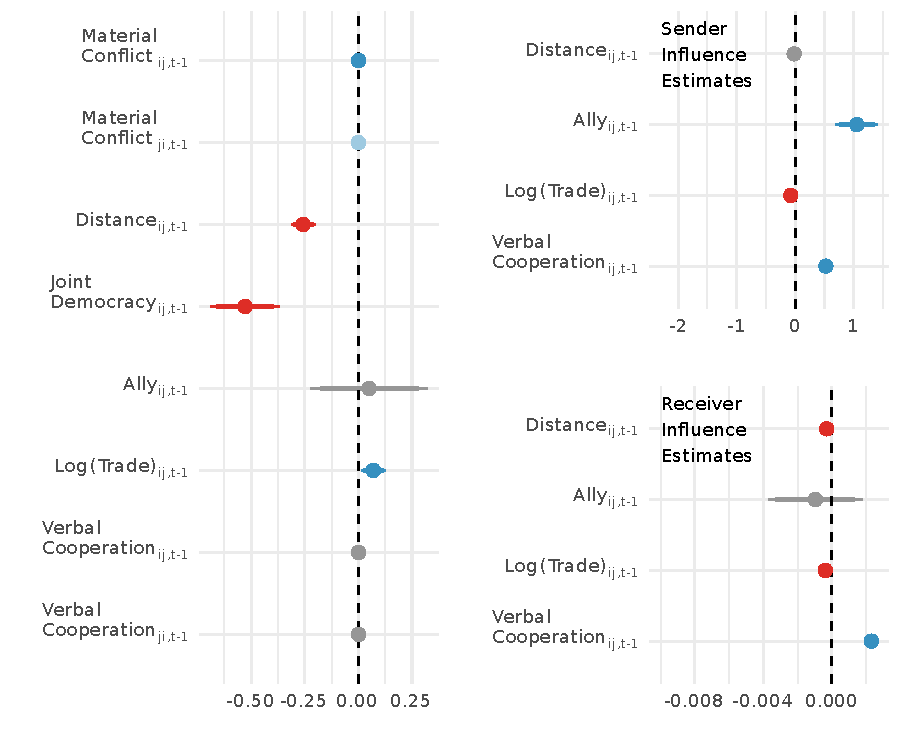
\includegraphics[width=1\textwidth]{figure5.pdf}
	\caption{Left-most plot shows results for the direct effect parameters and the top-right plot represents results for the sender influence, and bottom-right receiver influence parameters. Points in each of the plots represents the average effect for the parameter and the width the 90 and 95\% confidence intervals. Dark shades of blue and red indicate that the parameter is significant at a 95\% confidence interval and lighter shades a 90\% confidence interval. Parameters that are not significant are shaded in grey.}
	\label{fig:correlConf}
\end{figure}
\FloatBarrier

The right-most plots focuses on sender (top) and receiver (bottom) influence patterns. Notably, the alliance sender influence parameter has a positive effect, indicating that countries tend to initiate greater levels of conflict with countries that their allies were fighting in the previous period. This finding is in line with arguments in the extant literature about the role that alliance relationships may play in leading to more conflict in the international system \citep{siverson:king:1980,leeds:2005}.

Additionally, countries are likely to send conflict to those with whom their verbal cooperation partners are initiating or increasing conflict with. This finding is interesting as it highlights that countries making cooperative statements regarding a particular country $i$, actually go beyond those statements in later periods to supporting $i$ by initiating conflict with those that $i$ was in conflict with. Trade flows, on the other hand, are associated with having a negative effect, implying that countries are not likely, and in fact somewhat unlikely, to follow their trading partners into conflict.

Receiver influence patterns are similarly determined. Trade flows and verbal cooperation have similar effects, though the interpretation here for trade is that countries are unlikely to be targeted by those that target their trading partners. Interestingly, the distance effect on the receiver influence side is more precisely measured, implying that geographically proximate countries are more likely to receive conflict from a similar set of countries.

\subsection*{Visualizing Dependence Patterns}

Based on the sender and receiver influence parameter estimates, Figure~\ref{fig:inflRel} provides a visual summary of the type of dependence patterns that are implied in the context of the material conflict model estimated in the previous section.

The linear combination of our influence parameter estimates ($\alpha$), and the design array containing sender influence variables ($w_{ijt}$) are used to visualize the sender dependence patterns between a pair of countries ($a_{ijt}$): $a_{ijt} = \alpha^{\top} w_{ijt}$. The resulting sender and receiver dependence pattern are shown in Figure~\ref{fig:inflRel} for June 2007.\footnote{A lengthier table of visualizations for additional time periods is shown in Figure~\ref{fig:inflRelLong} of the Appendix.} For the visualization on the left [right], edges between countries indicate that greater likelihood to send [receive] conflictual events to [from] the same countries. Countries are colored by their relative geographic position and node size corresponds to the number of influence relationships the country shares.

Since these dependence patterns are estimated directly from the model results that are presented in Figure~\ref{fig:correlConf}, the patterns implied by that model are manifest in these visualizations. One of the more notable findings from the sender influence model is the role that alliance relationships play, and this effect is striking. For example, the USA shares sender influence ties with a number of Western European countries such as Germany and the United Kingdom, the USA also is more likely to send conflict to actors that Australia, South Korea and Japan have engaged in material conflict with, and many of these countries are likely to do the same.

\vspace{-2mm}
\begin{figure}[ht]
	\centering
	\begin{tabular}{l}
		\scshape{\textbf{June 2007}} \\
		\scshape{\;\;\;\; Sender Dependence Patterns} \\
		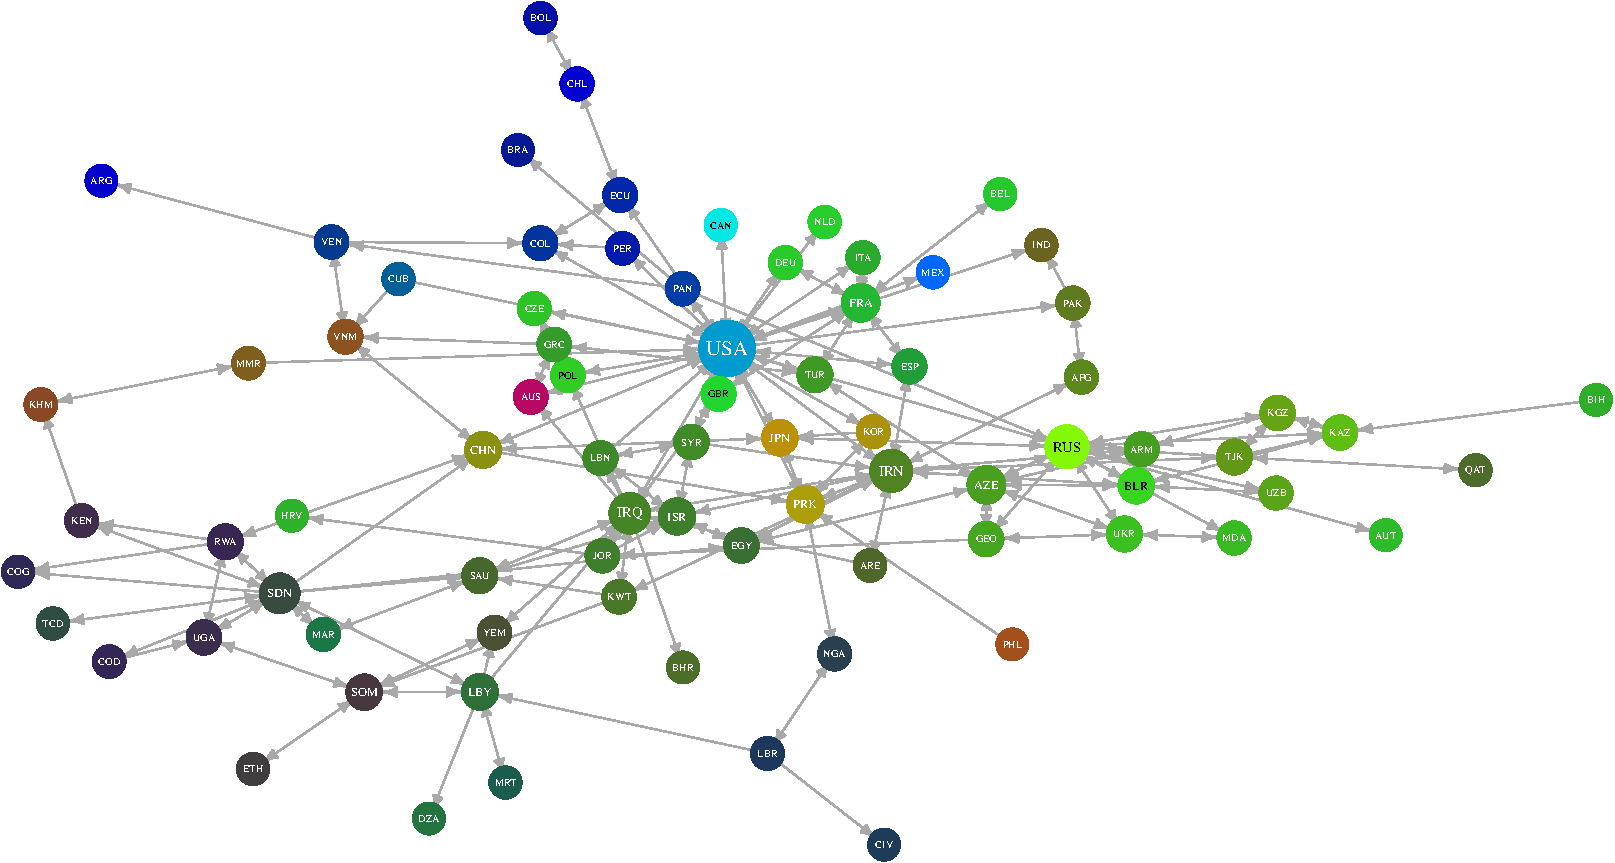
\includegraphics[width=.8\textwidth]{aInfl_2007_06_01.pdf} \\
		\scshape{\;\;\;\; Receiver Dependence Patterns} \\
		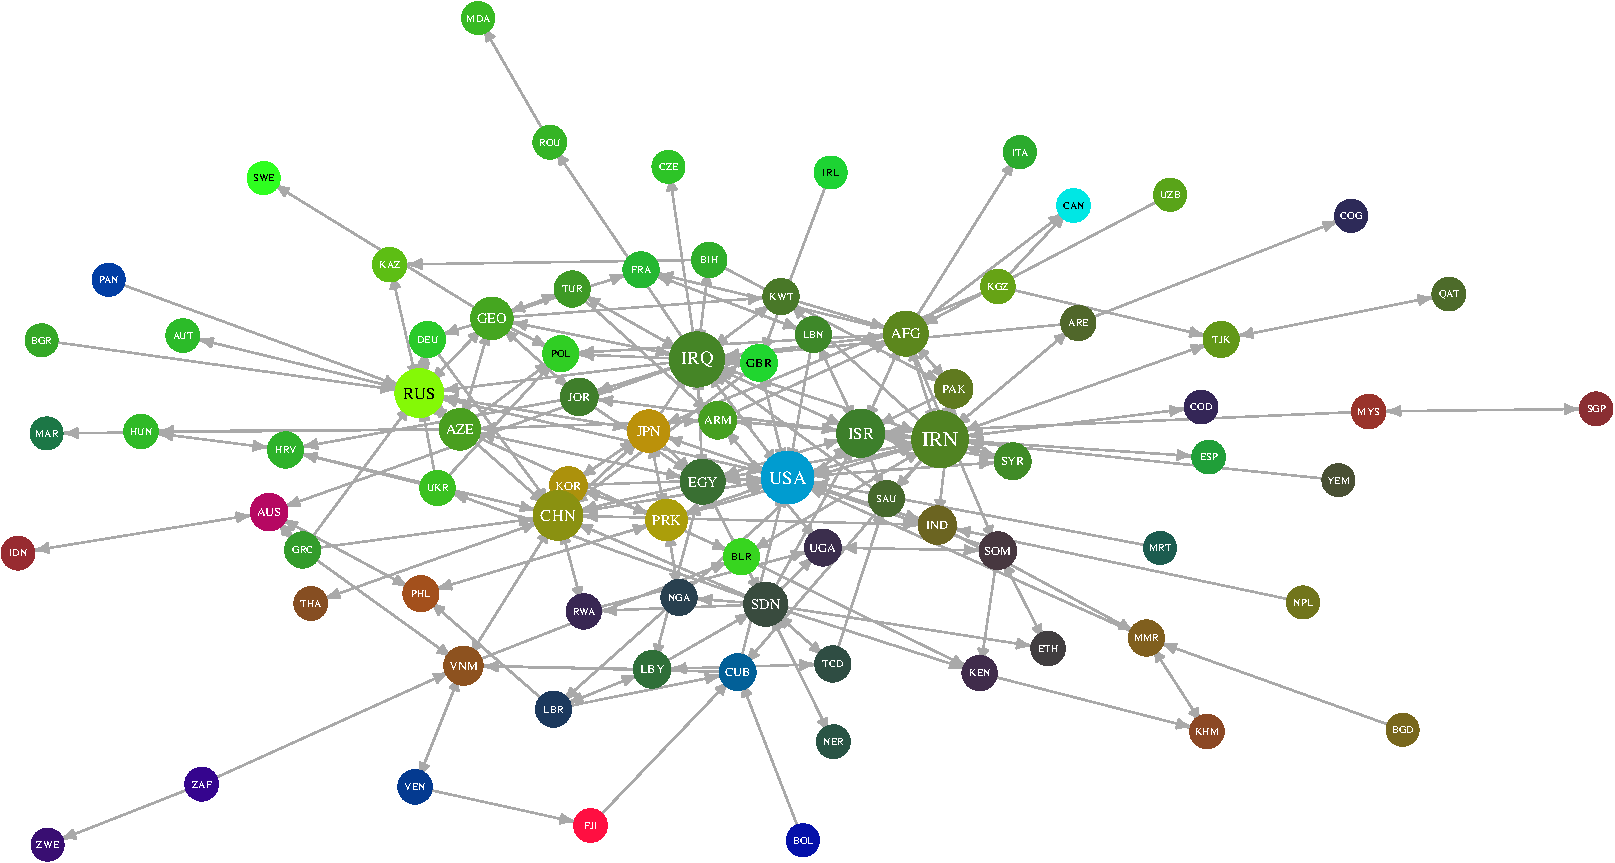
\includegraphics[width=.8\textwidth]{bInfl_2007_06_01.pdf} \\
	\end{tabular}
	\caption{Network visualization of influence patterns as estimated by the social influence regression model for June 2007. Nodes are colored by their relative geographic position and are sized by the number of influence relationships that they receive and send.}
	\label{fig:inflRel}
\end{figure}
\FloatBarrier

A predictor of receiver influence patterns is the distance between countries. Countries are more likely to be targeted by the same set of countries as their neighbors. This pattern manifests itself in the bottom visualization of Figure~\ref{fig:inflRel}, where we find clumps of countries, such as Iraq, Lebanon, and Jordan, clustering together.

\subsection*{Performance Comparison}

A common and important argument for employing a network based approach is that it aids in better accounting for the data generating process underlying relational data structures. Thus, in this case, the network approach should actually better predict conflict in an out-of sample test.\footnote{For more details on how one can develop predictions from the SIR model see the Appendix.} To put the performance of this model in context, we compare it to a standard GLM that does not account for dependence patterns in the network, but is similarly parameterized. Additionally, given the recent interest in machine learning methods as tools for prediction within the social sciences we compare the performance against a generalized boosted model (GBM).

Boosting methods have become a popular approach in the machine learning to ensemble over decision tree models in a sequential manner. At each iteration, a new model is trained with respect to the error of the ensemble at that point. \citet{friedman:2001} greatly extended the learning procedure underlying boosting algorithms, by modifying the approach to choose new models at every iteration so that they would be maximally correlated with the negative gradient of some loss function relevant to the ensemble. In the case of a squared-error loss function, this would correspond to sequentially fitting the residuals. We use a generalized version of this model developed by \citet{ridgeway:2012} that extends this framework to the estimation of a variety of distribution types---in our case, a Poisson regression model. In general, these types of models have been shown to give substantial predictive advantage over alternative methods, such as GLM, and should provide a useful point of comparison.\footnote{The $\sf{R}$ \pkg{gbm} package on CRAN implements this estimator \citep{ridgeway:2012}.}

To compare these approaches we first utilize a cross-validation procedure. This involves first randomly dividing $T$ time points in our relational array into $k=10$ sets and within each set we set randomly exclude five time slices from our material conflict array. We then run our models and predict the five missing slices from the estimated parameters. Proper scoring rules are used to compare predictions. Scoring rules evaluate forecasts through the assignment of a numerical score based on the predictive distribution and on the actual value of the dependent variable. \citet{czado:etal:2009} discuss a number of such rules that can be used for count data: Brier, Dawid-Sebastiani, Logarithmic, and Spherical scores.\footnote{Details are provided in the Appendix.} For each of these rules, lower values on the metric indicate better performance.

\begin{figure}[ht]
	\centering
	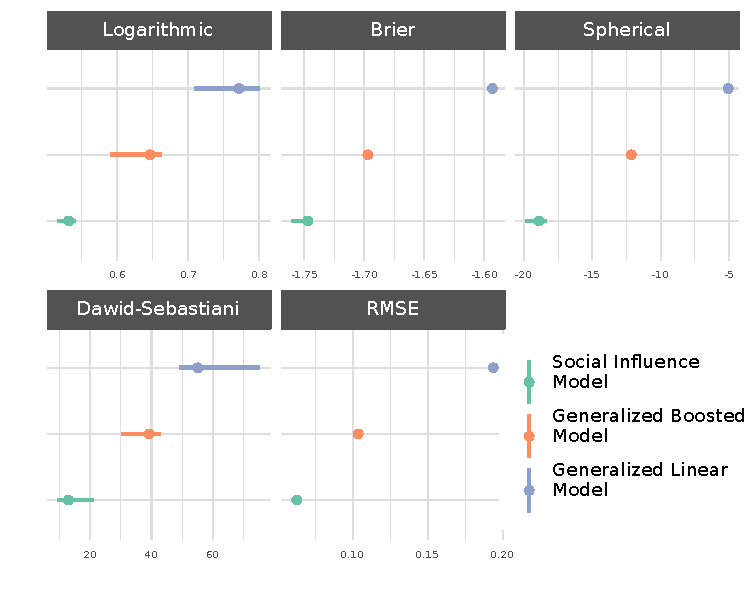
\includegraphics[width=.8\textwidth]{figure7.pdf}
	\caption{Performance comparison based on randomly excluding time slices from the material conflict array. Colors designate the different models, and the average score across the 10-fold cross validation is designated by a circle and the range by a horizontal line.}
	\label{fig:predCompareRandom}
	\end{figure}
\FloatBarrier

Figure~\ref{fig:predCompareRandom} illustrates differences in the performance between the social influence model, GLM, and GBM across the scoring rules mentioned above and a more standard metric, the RMSE. In the case of each of these metrics we find GLM performs the worst and that the social influence model performs the best.

We also assess the predictive accuracy of our models in a forecasting context. We perform such an exercise as well by dividing up our sample into a training and test set, where the test set corresponds to the last $x$ periods in the data that we have available. We vary $x$ from two to five. For instance, when $x=5$ we are leaving the last five years of data for validation. Results for this analysis are shown in Figure~\ref{fig:predCompareTime} and there again we find that the social influence model has better out of sample predictive performance than the alternatives we test here.

\begin{figure}[ht]
	\centering
	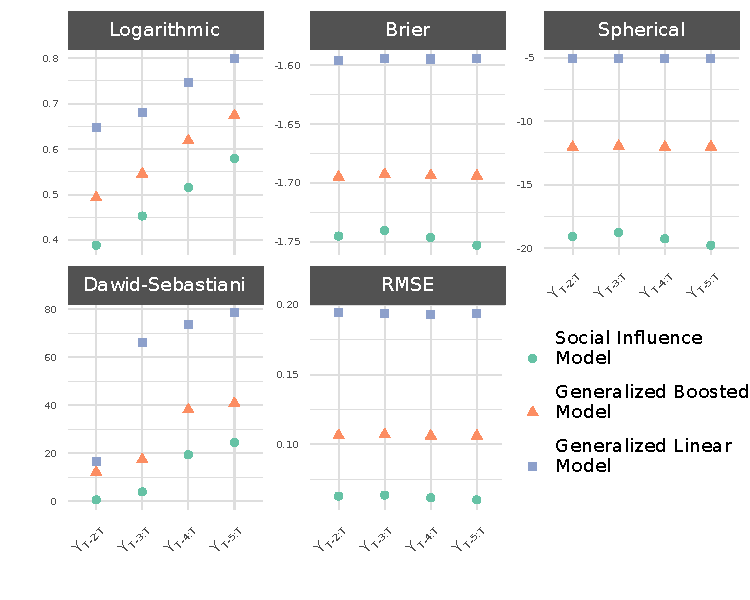
\includegraphics[width=.8\textwidth]{figure8.pdf}
	\caption{Performance comparison based on randomly excluding the last two to five periods of the material conflict array. Colors and shapes designate the different models, and the score when excluding $x$ number of periods is shown.}
	\label{fig:predCompareTime}
	\end{figure}
\FloatBarrier
